\documentclass{beamer}
\usepackage[utf8]{inputenc}
\usepackage[export]{adjustbox}
\usepackage{hyperref}
\hypersetup{
	colorlinks=true,
	urlcolor=adcorange,
	linkcolor=adcblue
}

\usetheme{Madrid}

\title{Let's make a todo list app with React Native!}
\subtitle{First workshop!}
\author{Nathaniel Budijono}
\date{January 25, 2022}
\institute{UMN ADC}

\definecolor{adcblue}{RGB}{115,203,255}
\definecolor{adcorange}{RGB}{242,114,0}

\setbeamercolor{palette primary}{fg=white,bg=adcblue}
\setbeamercolor{palette secondary}{fg=adcorange,bg=white}
\setbeamercolor{structure}{fg=adcblue,bg=white}
\setbeamercolor{title in head/foot}{fg=adcblue,bg=white}
\setbeamercolor{date in head/foot}{fg=gray,bg=white}
\setbeamercolor{palette tertiary}{fg=white,bg=adcorange}

\begin{document}

\begin{frame}
    \titlepage
    \includegraphics[width=0.25\textwidth, right]{figs/ADC_Logo_Blue.png}
\end{frame}

\begin{frame}{Logistics...}
	Streaming
	\begin{itemize}
		\item \href{https://z.umn.edu/adc-zoom}{https://z.umn.edu/adc-zoom}
		\item Recordings will be posted as unlisted YouTube videos as linked at \href{https://adcumn.org/meetings}{https://adcumn.org/meetings}
	\end{itemize}

	\bigskip\pause

	In-person
	\begin{itemize}
		\item Tuesdays 6-7pm
		\item Tate Hall 120
	\end{itemize}
\end{frame}

\begin{frame}{Officer openings!}
	\begin{itemize}
		\item Workshop instructors
	\end{itemize}

	\bigskip

	DM us on the discord!

	\bigskip

	\href{https://z.umn.edu/ADCdiscord}{https://z.umn.edu/ADCdiscord}
\end{frame}

\begin{frame}{Guide}
	We will be following this guide: \href{https://github.com/ADC-UMN/todotorial}{https://github.com/ADC-UMN/todotorial}. Feel free to go ahead of the workshops at your own pace.
\end{frame}

\begin{frame}{What is React?}
	React is a \emph{web application framework}. 

	\bigskip\pause
	
	It is \emph{declarative}. The building blocks are \emph{components}, which may be \emph{functional} or \emph{class components}.
\end{frame}

\begin{frame}{React class components}
	\centering
	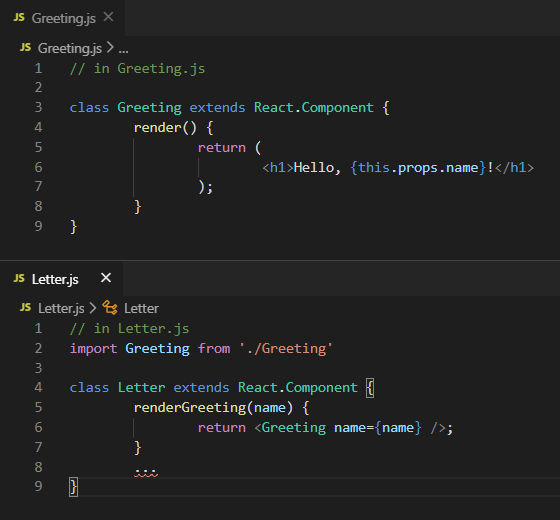
\includegraphics[width=0.7\textwidth]{figs/class-components.png}
\end{frame}

\begin{frame}{State}
	\centering
	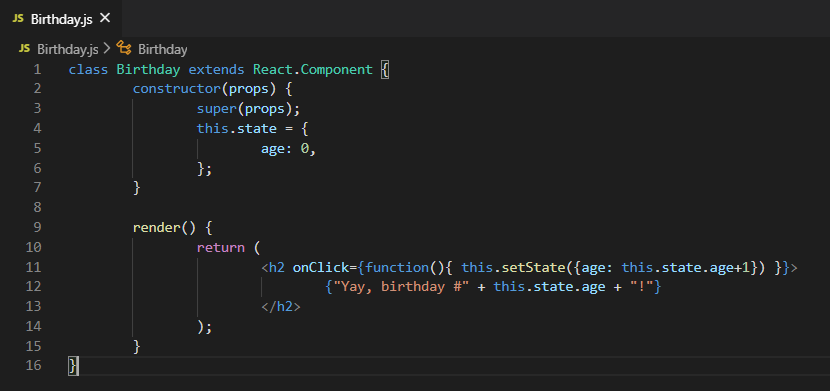
\includegraphics[width=0.9\textwidth]{figs/state.png}
\end{frame}

\begin{frame}{What is React Native?}
	React Native allows you to write \emph{cross-platform} React code instead of a \emph{native} codebase for each platform. However, you cannot use HTML. Instead,
	there are native component libraries for you to use.

	\bigskip\pause

	\centering
	
\includegraphics[width=0.8\textwidth]{figs/expo.png}
\end{frame}

\begin{frame}{Built-in components}
	\centering
	\begin{tabular}{|c|c|c|c|}
		\hline
		\textbf{React Native} & \textbf{Android} & \textbf{iOS} & \textbf{HTML} \\
		\hline
		\texttt{<View>} & \texttt{<ViewGroup>} & \texttt{<UIView>} & \texttt{<div>} \\
		\texttt{<Text>} & \texttt{<TextView>} & \texttt{<UITextView>} & \texttt{<p>} \\
		\texttt{<Image>} & \texttt{<ImageView>} & \texttt{<UIImageView>}  & \texttt{<img>} \\
		% \texttt{<TextInput>} & \texttt{<EditText>} & \texttt{<UITextField>} & \texttt{<input type="text">} \\
		\hline
	\end{tabular}
	
	\bigskip\pause

	See \href{https://reactnative.dev}{https://reactnative.dev} for more.
\end{frame}

\begin{frame}{Getting started}
	Snack allows you to edit and test your React Native apps in the browser at \href{https://snack.expo.io}{https://snack.expo.io}.

	\bigskip\pause

	You should instead use the Expo command line interface (CLI) so that you can build your app locally and upload it for distribution.
\end{frame}

\begin{frame}{Installing Node.js}
	Node is a version of JavaScript that can run outside of the browser. It is required for React Native.

	\bigskip\pause

	Go to \href{https://nodejs.org/en/download/}{https://nodejs.org/en/download/} to install.

	\bigskip\pause

	Confirm your installation and Node version with \texttt{node -v}.
\end{frame}

\begin{frame}{Installing the Expo CLI}
	Now that we have Node, we use the Node Package Manager (NPM) to install Expo's CLI.

	\bigskip\pause

	Run \texttt{npm install -g expo-cli}. \pause You can now create a template for a new project with \texttt{expo init} and test it with \texttt{expo start}.
\end{frame}

\begin{frame}{A look at what's ahead}
	\begin{enumerate}
		\item Components, Styling, and Testing
		\item Data Manipulation and State Handling
		\item Persistent Lists using AsyncStorage
		\item Deployment to Google Play Store
	\end{enumerate}

	\bigskip\pause

	Here's the finished product: \href{https://snack.expo.dev/@nathanielbd/todotorial}{https://snack.expo.dev/@nathanielbd/todotorial}. \pause What data should be kept track of using the state?
\end{frame}

\end{document}